\section{Introduction}
\label{sec:intro}

Epidemic modeling is an effective mathematical tool widely adopted in many domains to quantify the spreading dynamics of processes intertwined with large-scale networks~\cite{Vynnycky2010}. It serves as a viable framework for analyzing information diffusion in social networks~\cite{Dadlani2017}, cascading failure in power grids~\cite{Korkali2017}, secure routing in communication networks~\cite{Cheng2017}, and digital virus spreading in wireless mobile networks~\cite{Yang2018}. Dynamical models at the network scale can be broadly classified into two types: \emph{deterministic} and \emph{stochastic}. In deterministic models, the network is divided into smaller groups, each representing a specific stage of the epidemic. Such models, often formulated as differential equations (in continuous time) or difference equations (in discrete time), abstract what happens on the average at the network level. In contrast, a stochastic model is formulated as a stochastic process which in turn, is a set of random variables, $X(t;\varpi) \!\equiv \! X(t)$, defined as $\{X(t;\varpi)| t \!\in T~\textrm{and}~\varpi \!\in \!\Omega\}$ where $T$ and $\Omega$ represent time and a sample space, respectively. The solution of a stochastic model is a probability distribution for each of the random variables. Such models allow follow-up of each node in the network randomly~\cite{Brauer2001,Britton2010}.

Evolution of natural and man-made networks in both scale and complexity has triggered interdisciplinary research on characterizing the dynamics of stochastic processes spreading over them. 
Similar to the spreading of pathogens in biological systems, the virulence of spreading processes depends not only on the infection rate of each node, but also on the connectivity of the underlying network structure~\cite{Mieghem2014}. Increase in computational power over recent years has revealed the existence of heterogeneous and multi-faceted relations in the description of various diffusion processes~\cite{Newman2018}. %Limited mainly by memory space, the integration of such complex features in understanding the course of epidemic outbreaks using sophisticated simulation tools becomes time demanding as the network grows in size. 
The time taken to project the spreading pattern is important in devising effective countermeasures to prevent any potential outbreaks.
\begin{figure}[t!]
    \begin{center}
    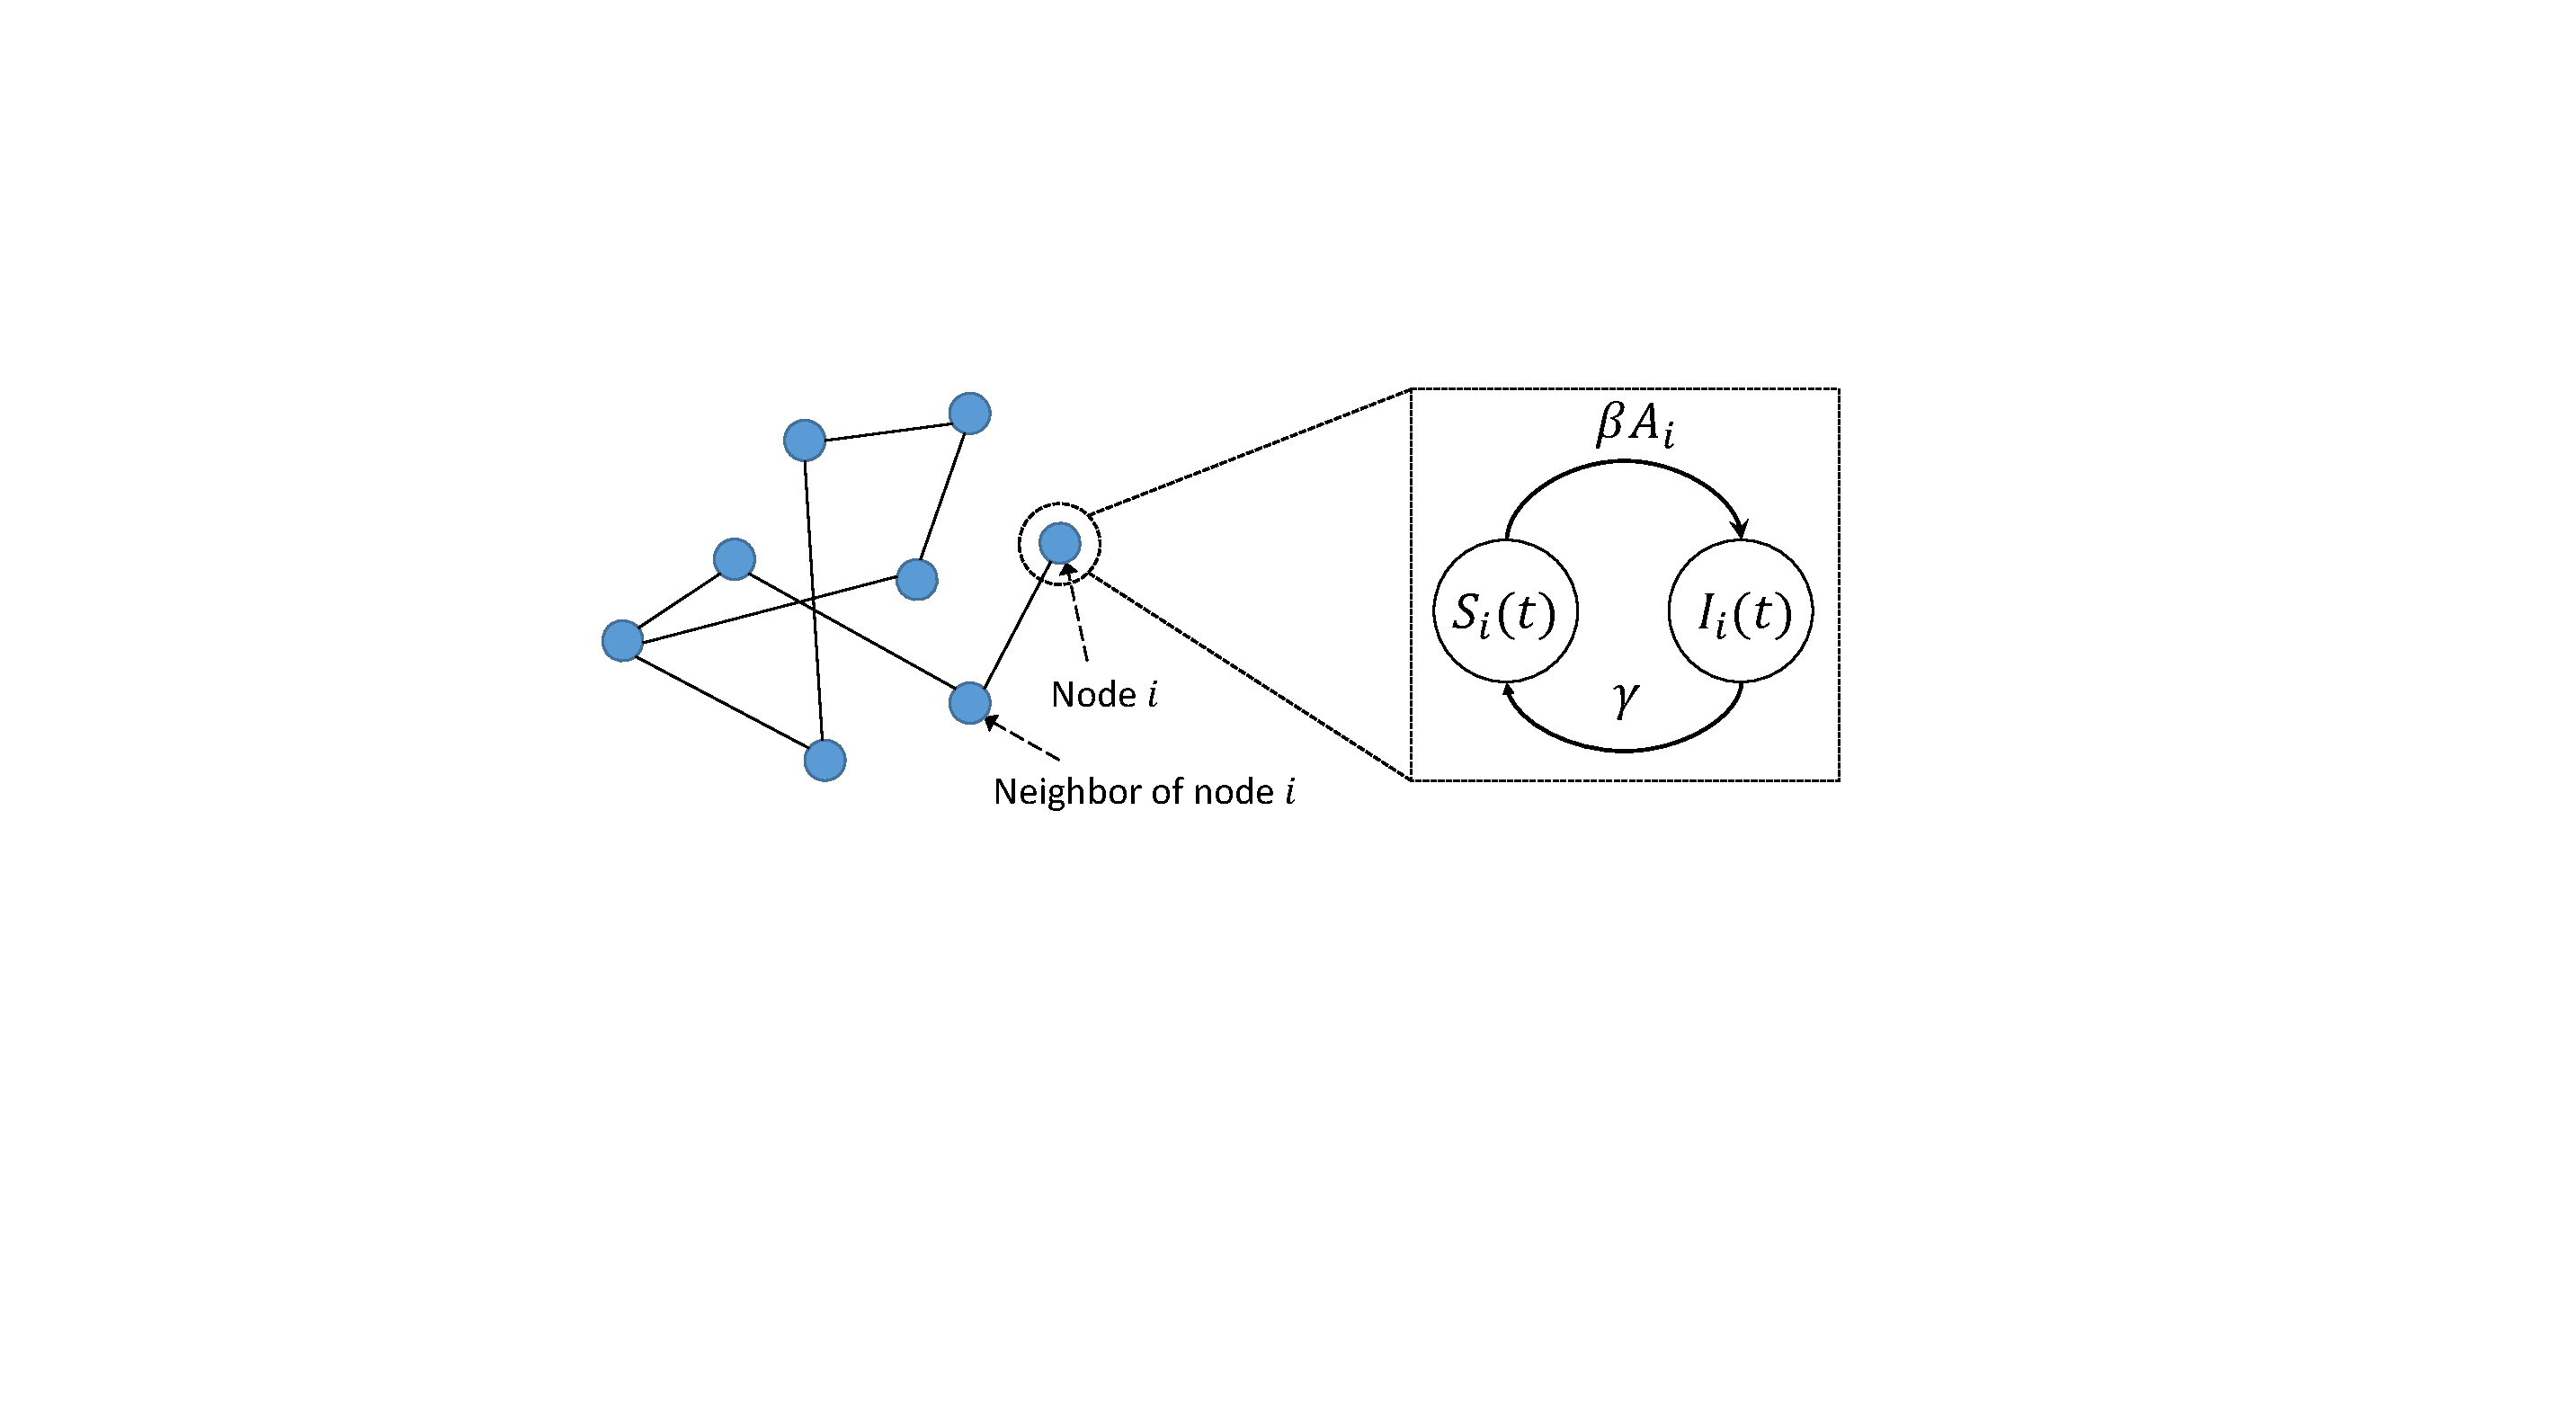
\includegraphics[width=0.8\columnwidth]{Figures/SIS.pdf}
    \caption{Schematic of the SIS model where $A_i$ denotes the direct neighbors of node $i$ in the network adjacency matrix $A$.} 
    \label{figure:sis}
    \end{center}
    \vspace{-5mm}
\end{figure}

We propose a network-on-chip (NoC) model supported on a reconfigurable platform called StocNoC to accelerate the epidemic projection of the spreading model. Due to its inherent parallelism, hardware implementation may significantly outperform pure software implementation especially due to the concurrent friendly nature of the model. The model is easily scalable to support larger network sizes, only limited by the resource availability of the target FPGA devices. Recent introduction of FPGA-accelerators in the cloud environment is especially encouraging in this regard, where users can choose the target device and scale it based on their computing requirements~\cite{Parimal2018}. Since the cloud-model charges users based on the target platform type and their running time, accelerated computation can significantly reduce the cost of computation. With minor modifications, the proposed platform can be used for hardware acceleration of other epidemic spreading models as well as spreading dynamics in contact networks in general.

The remainder of this paper is organized as follows. Section~\ref{sec:related} discusses the background of epidemic models and related works. Section~\ref{sec:architecture} presents the detailed architecture of the proposed hardware platform. Section~\ref{sec:results} discusses the hardware implementation results and the comparison with corresponding software implementation and Section~\ref{sec:conclusion} finally concludes the paper and gives future research directions.
